\documentclass[a4paper,10pt]{article}
\usepackage[utf8]{inputenc}
\usepackage{amsmath}
\usepackage{amsfonts}
\usepackage{breakurl}
\usepackage{indentfirst}
\usepackage{graphicx}
\usepackage{enumerate}
\usepackage[breaklinks, hidelinks]{hyperref}
\usepackage{url}
\usepackage{booktabs}
\usepackage{multirow}

\usepackage[textwidth=15cm,textheight=24cm]{geometry}


\newcommand{\vect}[1]{\ensuremath{\boldsymbol{#1}}}
\newcommand{\ddd}{\ensuremath{\,\mathrm{d}}}
\newcommand{\dd}{\mathrm{d}}
\newcommand{\Var}{\mathrm{Var}}
\newcommand{\pravYi}{P(Y_i|\alpha, \beta, \epsilon_i)}
\newcommand{\pravY}{P(\boldsymbol{Y}|\alpha, \beta, \epsilon_i)}
\newcommand{\nsigma}{\frac{N}{\sigma^2}}
\newcommand{\arpxsq}{\overline{(X^2)}}
\newcommand{\sigman}{\frac{\sigma^2}{N}}
\newcommand{\jmenovatel}{ \arpxsq - \overline{X}^2}
\usepackage{amsmath}


\title{ZDC photomultipliers gain analysis 2018}
\author{Miroslav Šimko, Lukáš Kramárik, Jan Vaněk}
\date{}



\begin{document}

\maketitle

\section{Gain curves}
STAR Zero Degree Calorimeters (ZDC) use the photomultiplier (PMT) assemblies H2431-50~\cite{H2431} from Hamamatsu, with the photomultiplier tube R2083~\cite{R2083}. The gain on the PMTs follows the power law dependence
\begin{equation} \label{power_law}
G = \left(\frac{U}{U_0} \right)^X
\end{equation}
with the high voltage $U$ on the dinodes where $G$ is the measured gain where the coefficients $U_0$ and $X$ are PMT-dependent and have to be extracted from measurement for each PMT separately.

\begin{figure}[htb]
\begin{center}
% 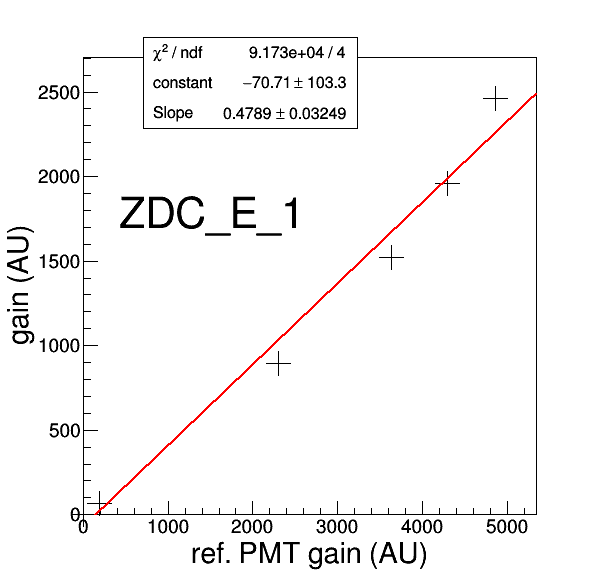
\includegraphics[width=.49\textwidth]{img/ZDC_E_1.pdf}
% 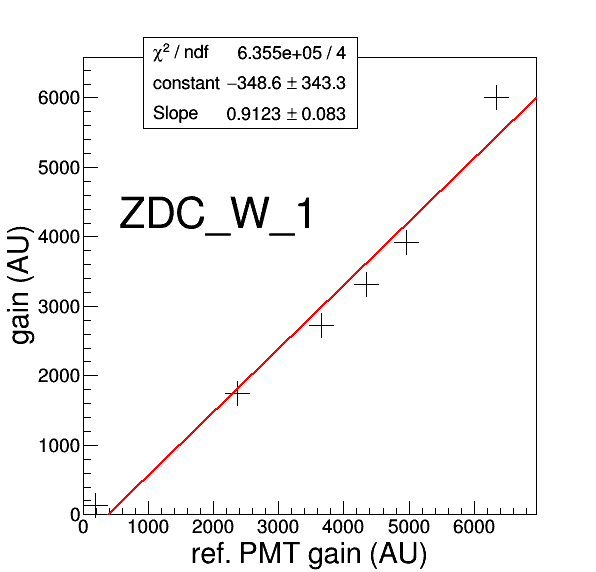
\includegraphics[width=.49\textwidth]{img/ZDC_W_1.pdf}\\
% 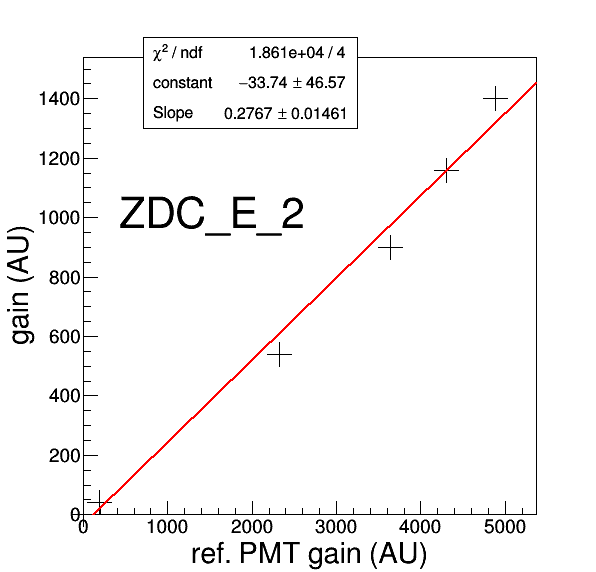
\includegraphics[width=.49\textwidth]{img/ZDC_E_2.pdf}
% 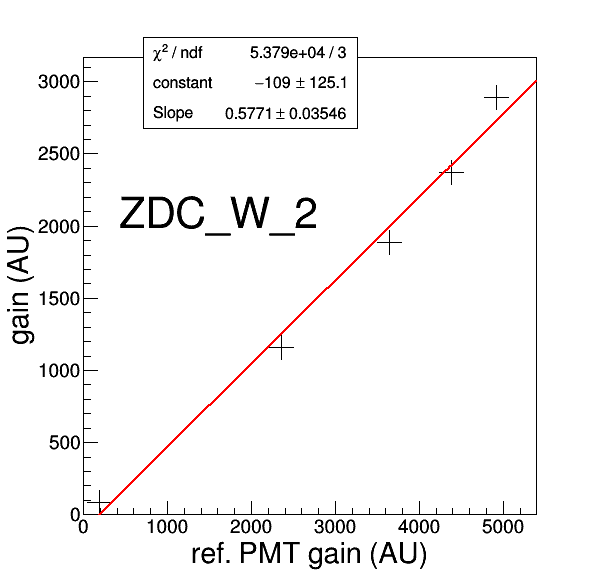
\includegraphics[width=.49\textwidth]{img/ZDC_W_2.pdf}\\
% 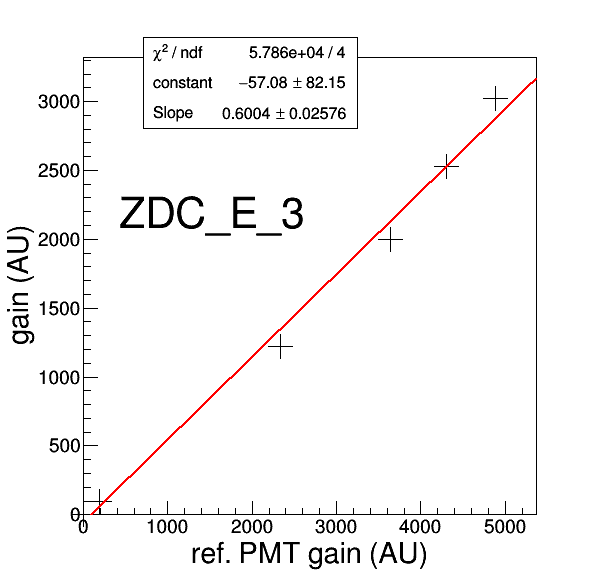
\includegraphics[width=.49\textwidth]{img/ZDC_E_3.pdf}
% 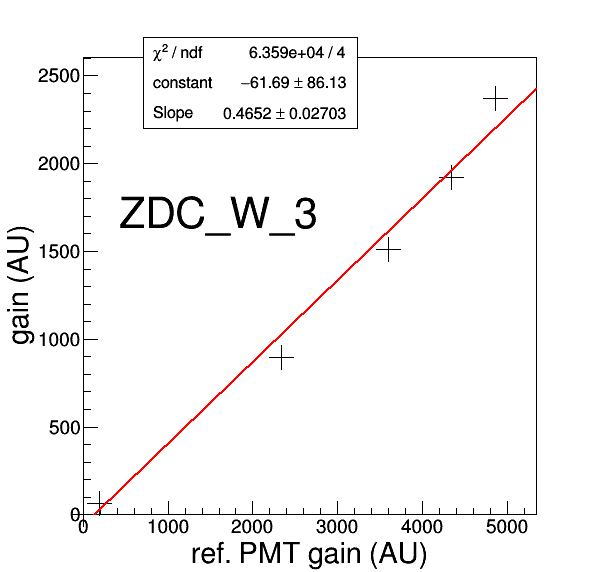
\includegraphics[width=.49\textwidth]{img/ZDC_W_3.pdf}
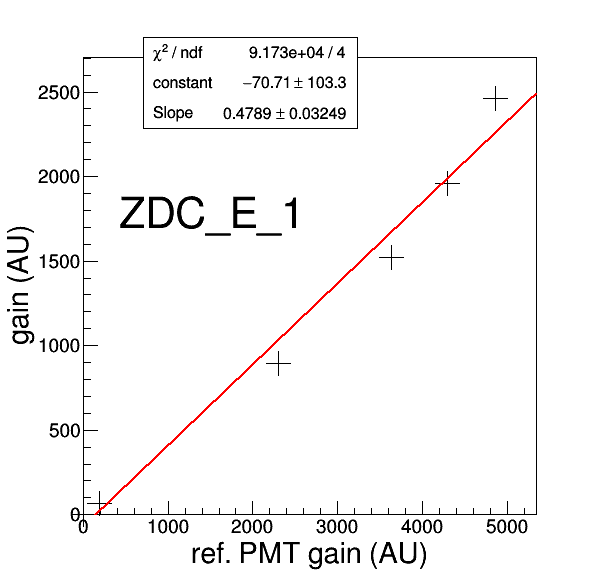
\includegraphics[width=.32\textwidth]{img/ZDC_E_1.pdf}
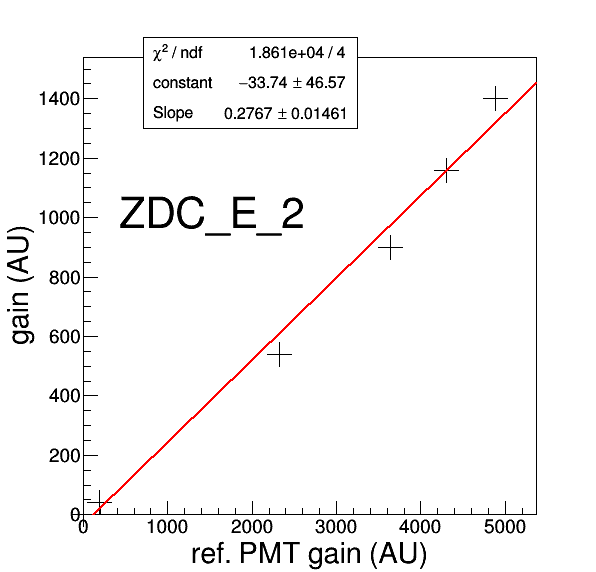
\includegraphics[width=.32\textwidth]{img/ZDC_E_2.pdf}
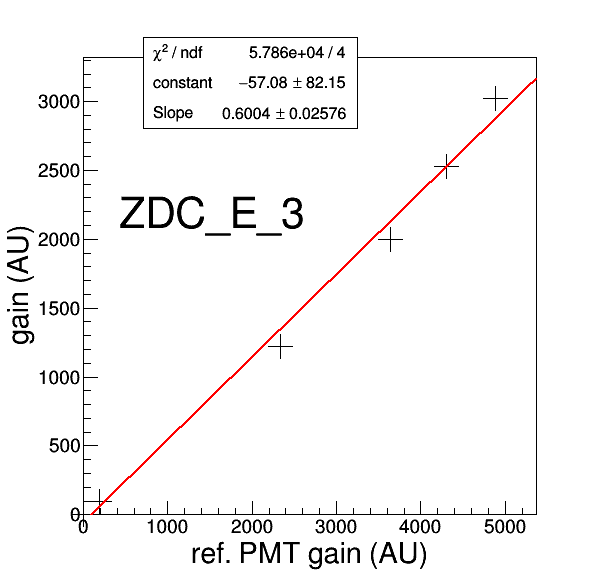
\includegraphics[width=.32\textwidth]{img/ZDC_E_3.pdf}\\
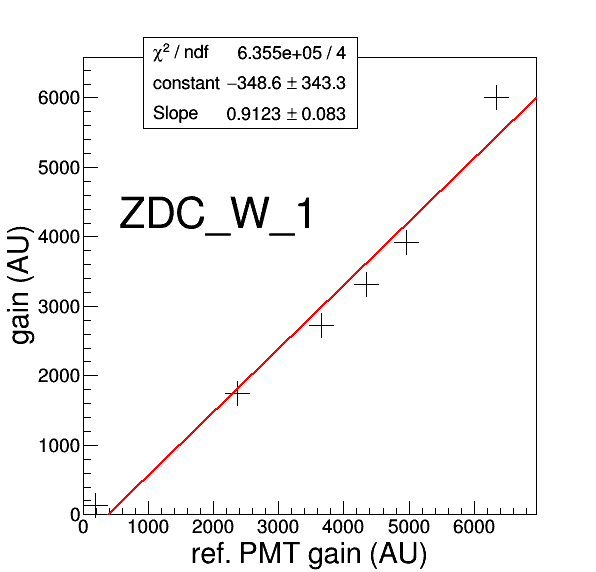
\includegraphics[width=.32\textwidth]{img/ZDC_W_1.pdf}
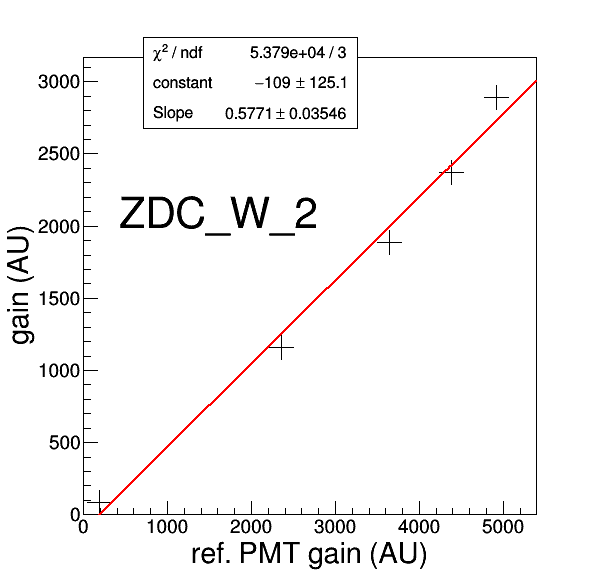
\includegraphics[width=.32\textwidth]{img/ZDC_W_2.pdf}
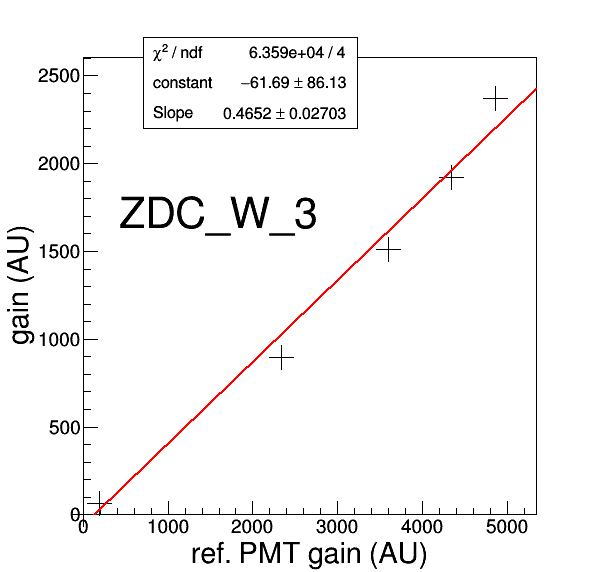
\includegraphics[width=.32\textwidth]{img/ZDC_W_3.pdf}
\end{center}
\caption{\label{gainCurves}Gain curves of ZDC photomultipiers. The measurement is described in more detail in~\cite{table} and~\cite{ZDC_PMT_presentation}.}
\end{figure}

We have measured the gain using a simple setup with a pulsing LED with controlled light output, the measured PMT, and a control PMT, all of them closed in a dark box. The amplitude of the pulse from the PMT was measured via an oscilloscope. We measured the gain for 10 voltages between 2.1 kV and 3 kV, then we added 1 measurement at 3.4 kV to test whether the PMT starts showing saturation at high voltages\@. The resulting gains follow nicely the power law \eqref{power_law} as can be seen in Figure~\ref{gainCurves}. No saturation of the gain was observed in this measurement, however, we have encountered saturation with higher frequency of the light input. The fitted constants $U_0$ and $X$ are summarized in Table~\ref{gainTable}. The whole measurement is described in more detail in~\cite{table} and~\cite{ZDC_PMT_presentation}.


\begin{table}[htb]
\caption{\label{gainTable}Gain curve constants.}
\begin{center}
\begin{tabular}{lcr@{ $\pm$ }lr@{ $\pm$ }l}
\toprule
&&\multicolumn{2}{c}{$U_0$ (V)}&\multicolumn{2}{c}{$X$ ()}\\
\midrule
East:&1&1376&5&6.60&0.03\\
     &2&1463&8&6.44&0.05\\
     &3&1289&4&6.50&0.02\\
\midrule
West:&1&1176&4&6.13&0.02\\
     &2&1259&4&6.09&0.02\\
     &3&1265&4&5.77&0.02\\
\bottomrule
\end{tabular}
\end{center}
\end{table}

Using the gain dependence \eqref{power_law} and the constants from Table \ref{gainTable}, we can obtain the gain at the set voltages in 2016 and 2017 running for the light output of our LED\@. These voltages were calibrated on the single-neutron peak (SNP) in 2016 as can be found in Chapter~4 in~\cite{ZDC_ops_manual}\@. 

The measured gains are in Table~\ref{glassTable} which also shows the ratio $G/G_\text{West3}$ of the gain of the corresponding tower to the tower West3 which had the best performance of the measured PMTs\@. This ratio can tell us something about the light registered by the PMTs. Higher gain ratios can mean 1 or, perhaps, a combination of the following factors:
\begin{enumerate}
\item The fibers leading to the PMTs are more radiation-damaged or have a worse surface and, therefore, transmit less light.
\item The gain of the corresponding PMT has dropped more than others in 2016 and 2017.
\item The calibration set the PMT's voltage too high as, e.g.\ for the 3rd towers, the SNP method is not very accurate. 
\end{enumerate}


\begin{table}[htb]
\caption{\label{glassTable}Gains comparison with constant light exposure.}
\begin{center}
\begin{tabular}{lcccc}
\toprule
&&$U_\text{2016}$ (V)&$G$ (AU)& $G/G_\text{West3}$ ()\\
\midrule
East:&1&2540&57&0.49\\
&2&3000&102&0.87\\
&3&2557&86&0.73\\
\midrule
West:&1&2558&117&1\\
&2&2748&116&1\\
&3&3000&146&1.25\\
\bottomrule
\end{tabular}
\end{center}
\end{table}

In the scenario 1 is true or it is the dominant factor in the gain difference, we can conclude that the fibers on the West side are considerably worse than in the East and the tower with the worse light output is the West3\@ which also has one of the worst PMTs. This opens possibilities for swapping of the PMTs.

\section{Voltage estimates for 2018}
The gain from the ZDC photomultipiers is dropping each year. This effect occurs in between high-energy running, therefore this is not expected to be luminosity-dependent. However, luminosity dependence is also considered here.

In table \ref{voltsTable} set voltages from 2014 ($U_{2014}$) and 2016 ($U_{2016}$) are shown. All of the voltages were obtained from SNP calibration described in \cite{calib2014} and in Chapter 4 of \cite{ZDC_ops_manual}\@. If we consider that the gain lowers with time at a constant rate
\begin{equation}
G_{2018} = G_{2016} + (G_{2016} - G_{2014})\,,
\end{equation}
we easily get the result for voltages from the dependence \eqref{power_law}
\begin{equation}
U_{2018}^\text{linear} = (2 U_{2016}^X - U_{2014}^X)^{1/X}\,.
\end{equation}
Since the STAR ZDC has been exposed to an unprecedented luminosity from Au+Au running in 2016 and p+p running at $\sqrt{s} = 500$~GeV, we have also considered a scenario where the gain decrease in 2016--2017 is 4$\times$ higher than in 2014--2015
\begin{equation}
G_{2018} = G_{2016} + 4(G_{2016} - G_{2014})\,,
\end{equation}
which we consider a conservative estimate. For the voltages we get
\begin{equation}
U_{2018}^{4\times} = (5 U_{2016}^X - 4 U_{2014}^X)^{1/X}\,.
\end{equation}

\begin{table}[htb]
\caption{\label{voltsTable}Voltages estimates for the year 2018.}
\begin{center}
\begin{tabular}{lccccc}
\toprule
&&$U_{2014}$ (V)&$U_{2016}$ (V)& $U_{2018}^\text{linear}$ (V)&$U_{2018}^{4\times}$ (V)\\
\midrule
East:&1&2471&2540&2600&2744\\
&\textbf{2}&2779&3000&\textbf{3157}&\textbf{3471}\\
&3&2353&2557&2698&2974\\
\midrule
West:&1&2532&2558&2583&2650\\
&2&2643&2748&2836&\textbf{3039}\\
&\textbf{3}&2671&3000&\textbf{3214}&\textbf{3619}\\
\bottomrule
\end{tabular}
\end{center}
\end{table}

The resulting voltages are written in Table~\ref{voltsTable}. The voltages in boldface exceed the maximum allowed voltage of the ZDC power supply and the corresponding PMTs will have to be replaced or swapped with other channels.





\begin{thebibliography}{10}
\bibitem{H2431} Hamamatsu, \textit{Photomultiplier tube assembly H2431-50}, \today, \url{https://www.hamamatsu.com/eu/en/product/alpha/P/3002/H2431-50/index.html}.
\bibitem{R2083} Hamamatsu, \textit{Photomultiplier tube R2083}, \today, \url{https://www.hamamatsu.com/us/en/R2083.html}.
\bibitem{table} M.\ Šimko, L.\ Kramárik, J. Vaněk, \textit{ZDC photomultipiers measurement table}, \today,\\ \url{https://docs.google.com/spreadsheets/d/1E0_PEfIwpkxFE8akk1zveQZgpWWD2qElOYhLvDSjPkg/edit?usp=sharing}.
\bibitem{ZDC_PMT_presentation} M.\ Šimko, L.\ Kramárik, J. Vaněk, \textit{ZDC PMT status}, February 26, 2018,
 \url{https://docs.google.com/presentation/d/1dRxTr7tnv7KC7v8NkkvprQo8QhEIIJN8mbcBwf5cAsI/edit?usp=sharing}.
\bibitem{spares_presentation} M.\ Šimko, L.\ Kramárik, J. Vaněk, \textit{Spare PMT for ZDC}, February 26, 2018, \url{https://docs.google.com/presentation/d/1XugTbF7yzF5O6N5T5vcKFjVigoiqAoXKdcchxtWM_uM/edit?usp=sharing}.
\bibitem{calib2014} Y.\ Xu et al. \textit{Physics Performance of the STAR Zero Degree Calorimeter at Relativistic Heavy Ion Collider}, \url{https://www.bnl.gov/isd/documents/94732.pdf}.
\bibitem{ZDC_ops_manual} M.\ Šimko, L.\ Kramárik, \textit{Zero Degree Calorimeter Operator’s
Manual}, 2017, \url{http://www.star.bnl.gov/~msimko/ZDCopsManual.pdf}.
\end{thebibliography}


\end{document}



